This work studies the internal mechanism of how long-context language models can utilize information at arbitrary locations within the input. 
Recent advances in long-context language modeling~\citep{claude, reid2024gemini, fu2024data} show inspiring results, particularly on the Needle-in-a-Haystack test~\citep{needleinhaystack}, which asks the model to precisely retrieve the information of a short sentence (the needle) within a long context (the haystack). 
Such capability is the basis of more advanced long-context tasks, which usually interleaves retrieval and reasoning in a multi-step fashion~\citep{kuratov2024search}. 
Based on extensive experiments across 4 model families, 6 model scales, and 3  types of finetuning,
we show that across the models' attention layers, there exist a small number of retrieval heads that search the information being asked, and redirect the relevant tokens from the input to the output. 
Activation of retrieval heads explains whether the output is factual or hallucinated. 
When such heads are activated, the model behaves faithful to the input document.
When they are not activated, or intentionally masked out in controlled experiments (Fig.~\ref{fig:retrieval_head}), the model cannot find the relevant information and hallucinate instead. 


\begin{figure*}[!t]
\small
  \centering
  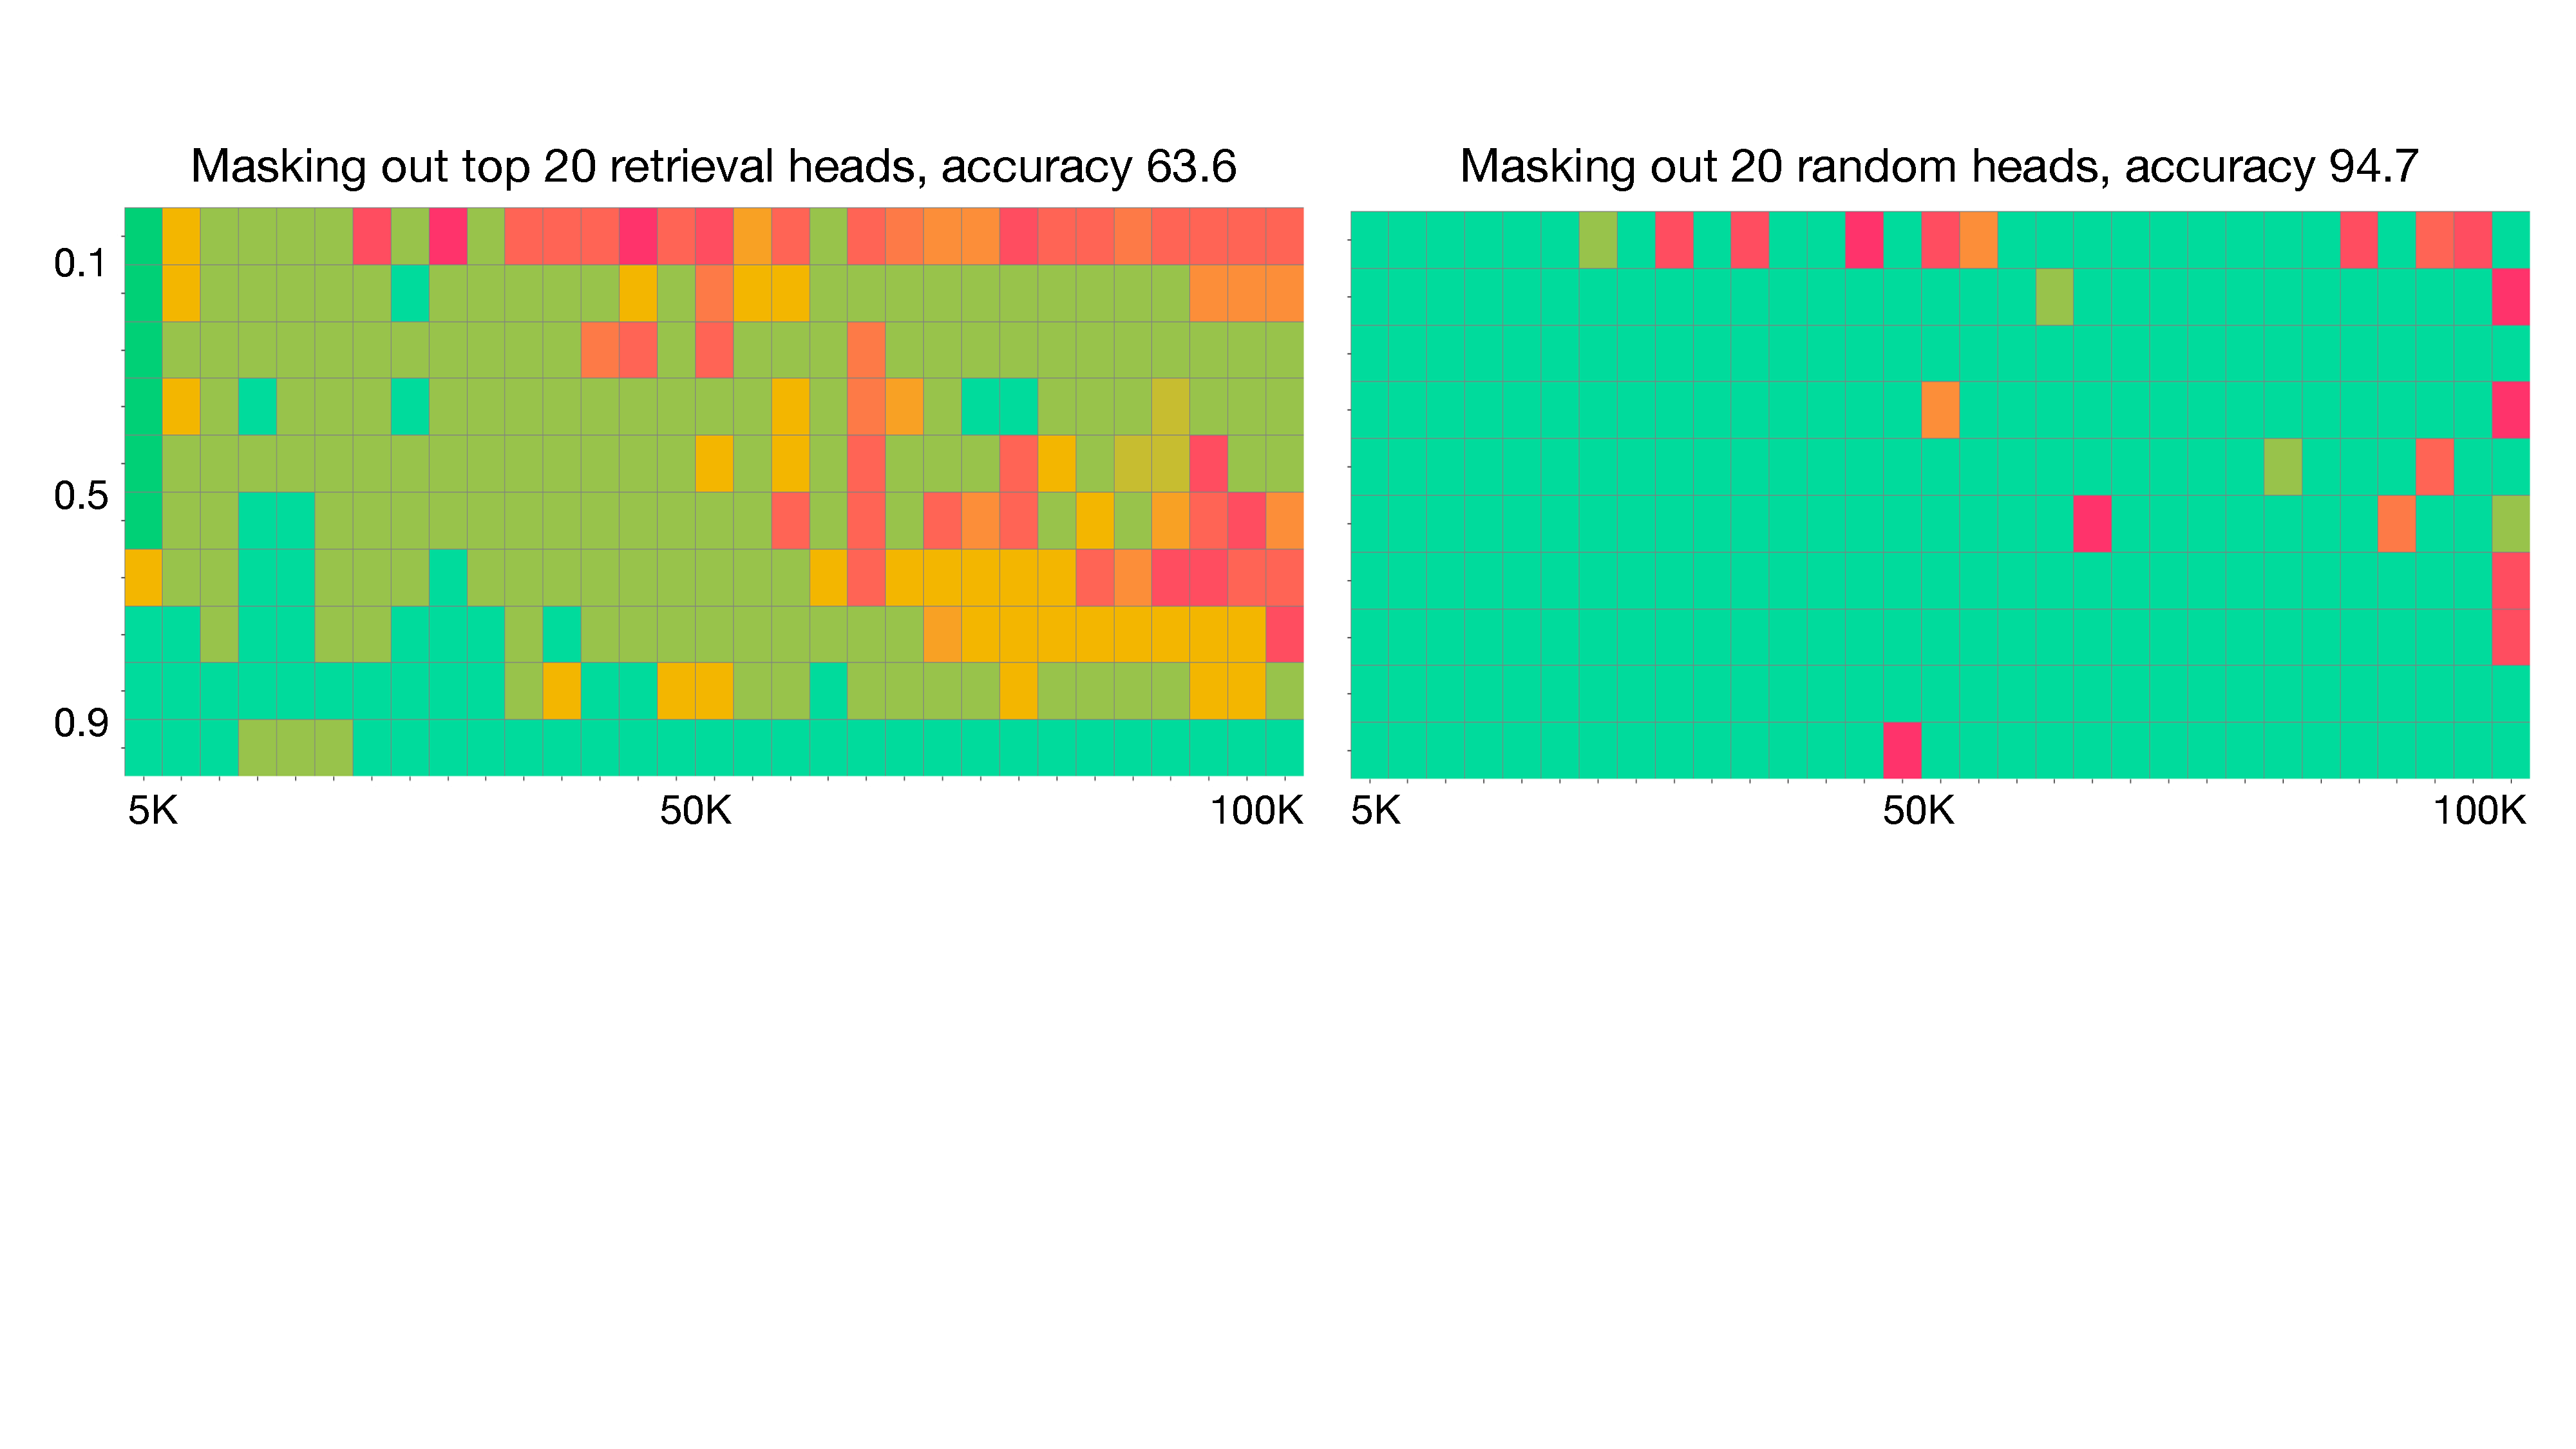
\includegraphics[width=\linewidth]{figures/retrieval_head.pdf}
  \caption{Retrieval heads are the heads that redirect information from the input to the output. Left: masking out the top retrieval heads of LLaMA 2 7B 80K, its Needle-in-a-Haystack performance drops significantly, and the model hallucinates during decoding. Right: masking out random non-retrieval heads does not influence the model's needle-in-a-haystack behavior. 
  We further note that the retrieval head only influence factuality but not the language capability: when they are masked, the model hallucinates by saying ``go to the beach'', which is still a fluent sentence, but not factual (as the correct answer is ``eating a sandwich at Dolores park.'').
  }
  \label{fig:retrieval_head}
\end{figure*}


% P2. Motivate retrieval head with what attention might be doing, the copy net, and induction head
The discovery of the retrieval head is motivated by the question of what the attention mechanism is doing when the model can or cannot find the given needle.
We take important inspiration from two existing works: the CopyNet~\citep{gu-etal-2016-incorporating} and the Induction Head~\citep{olsson2022context}.
The CopyNet is essentially a single-layer, single-head attention mechanism in the age of RNNs that copy-paste tokens from the input to the output.
Induction Heads~\citep{olsson2022context} are special heads within a multi-layer, multi-head attention network that implements an implicit program induction algorithm.
Combining the observation from the two works, we natually hypothesize that, just like induction heads are accountable for in-context learning, there might exist special heads that are accountable for information retrieval and implement a conditional copy-paste algorithm.

We design algorithms to detect retrieval heads within the transformer architecture (Sec.~\ref{sec:retrieval_head}), and conduct large-scale experiments to demonstrate important properties of them (Sec.~\ref{sec:properties}):
(1) retrieval heads are universal and sparse: for any model family (LLaMA~\citep{touvron2023llama}, Yi~\citep{young2024yi}, QWen~\citep{bai2023qwen} and Mistral~\citep{jiang2023mistral}), at any scale (6B, 14B, and 34B and 8$\times$7B), either base or chat, either dense or MoE, as long as the model can precisely recite the input information, they have a small number of retrieval heads (Fig.~\ref{fig:retrieval_head});
(2) they are intrinsic: the base model (e.g., LLaMA2 base) already contains retrieval heads (as a consequence of large-scale pretraining). Subsequent derivations, such as the long-context continue pretraining (LLaMA2 7B 80K),  chat fine-tuning (Qwen Chat), or even sparse upcycling~\citep{komatsuzaki2022sparse, jiang2024mixtral} uses the same retrieval heads as the base model (Fig.~\ref{fig:heat_map}); 
(3) they are dynamically activated according to the context: the strongest retrieval heads (e.g., 13 for LLaMA 2 7B) are always activated no matter what the required information is, while weaker retrieval heads  are activated on different parts of the required information; consequently these heads compensate each other's functionality: removing a subset of the heads, the model at least retrieve part of the required information;
(4) the retrieval heads are causal: 
say we put a needle "the best thing to do in San Francisco is to eat a sandwich in Dolores Park on a sunny day",
completely masking out retrieval heads, the model hallucinates (by saying the best thing is to visit Golden Gate bridge); 
partially masking out the heads, the model retrieves part of the needle (e.g., it gets the sandwich but forget the Dolores Park);
masking out random non-retrieval heads, the model still find full needle; 
when we do not mask the head yet the model still hallucinate in some cases, 
the retrieval heads are not activated. 
We further note that chain-of-thought reasoning also heavily relies on retrieval heads because the model needs to refer back the input information, indicating a complex relationship between the model's retrieval and reasoning capability.

The discovery of retrieval head has profound implications on long-context modeling:
(1) it marks a significant step forward in the field of mechanistic interpretability~\citep{bricken2023monosemanticity, olsson2022context} because for the first time we pin point a particular subnet implementing the conditional retrieval algorithm;
(2) it explains why certain context-compression methods fail to keep factuality (because they removes the retrieval head, e.g., in~\citealt{xiao2023efficient}), and suggests future research on KV cache compression~\citep{ge2023model, kang2024gear}, a key problem for deploying long-context models, should consider the influence of retrieval heads. 